\documentclass{beamer}

\usefonttheme{professionalfonts} % using non standard fonts for beamer
\usefonttheme{serif} % default family is serif

%\usepackage{hyperref}

%\usepackage{minted}

\usepackage{animate}

\usepackage{graphicx}

\def\Put(#1,#2)#3{\leavevmode\makebox(0,0){\put(#1,#2){#3}}}

\usepackage{color}

\usepackage{tikz}

\usepackage{amssymb}

\usepackage{enumerate}


\newcommand\blfootnote[1]{%

  \begingroup

  \renewcommand\thefootnote{}\footnote{#1}%

  \addtocounter{footnote}{-1}%

  \endgroup

}

\makeatletter

%%%%%%%%%%%%%%%%%%%%%%%%%%%%%% Textclass specific LaTeX commands.

 % this default might be overridden by plain title style

 \newcommand\makebeamertitle{\frame{\maketitle}}%

 % (ERT) argument for the TOC

 \AtBeginDocument{%

   \let\origtableofcontents=\tableofcontents

   \def\tableofcontents{\@ifnextchar[{\origtableofcontents}{\gobbletableofcontents}}

   \def\gobbletableofcontents#1{\origtableofcontents}

 }

%%%%%%%%%%%%%%%%%%%%%%%%%%%%%% User specified LaTeX commands.

\usetheme{Malmoe}

% or ...

\useoutertheme{infolines}

\addtobeamertemplate{headline}{}{\vskip2pt}



\setbeamercovered{transparent}

% or whatever (possibly just delete it)

\makeatother

\begin{document}
\title[DDCEL report]{A Scalable DCEL implementation}
\author[AC]{Andres Calderon}
\institute[Spring'20]{University of California, Riverside}
\makebeamertitle
\newif\iflattersubsect

\AtBeginSection[] {
  \begin{frame}<beamer>
    \frametitle{Outline} 
    \tableofcontents[currentsection]  
  \end{frame}
  \lattersubsectfalse
}

\AtBeginSubsection[] {
  \begin{frame}<beamer>
    \frametitle{Outline} 
    \tableofcontents[currentsubsection]  
  \end{frame}
}

\begin{frame}{Overlay operations}{CGAL implementation}
    \begin{itemize}
        \item  Extend the CGAL implementation to evaluate the overlay operators.
        \item Run validations with Phili dataset.
        \item Run experiments with CA dataset: 
        \begin{itemize}
            \item Cluster: 12 nodes, 8 cores each.
            \item Average of 10 runs.
        \end{itemize}
        
    \end{itemize}
\end{frame}

\begin{frame}{Experiment results}
    \centering
	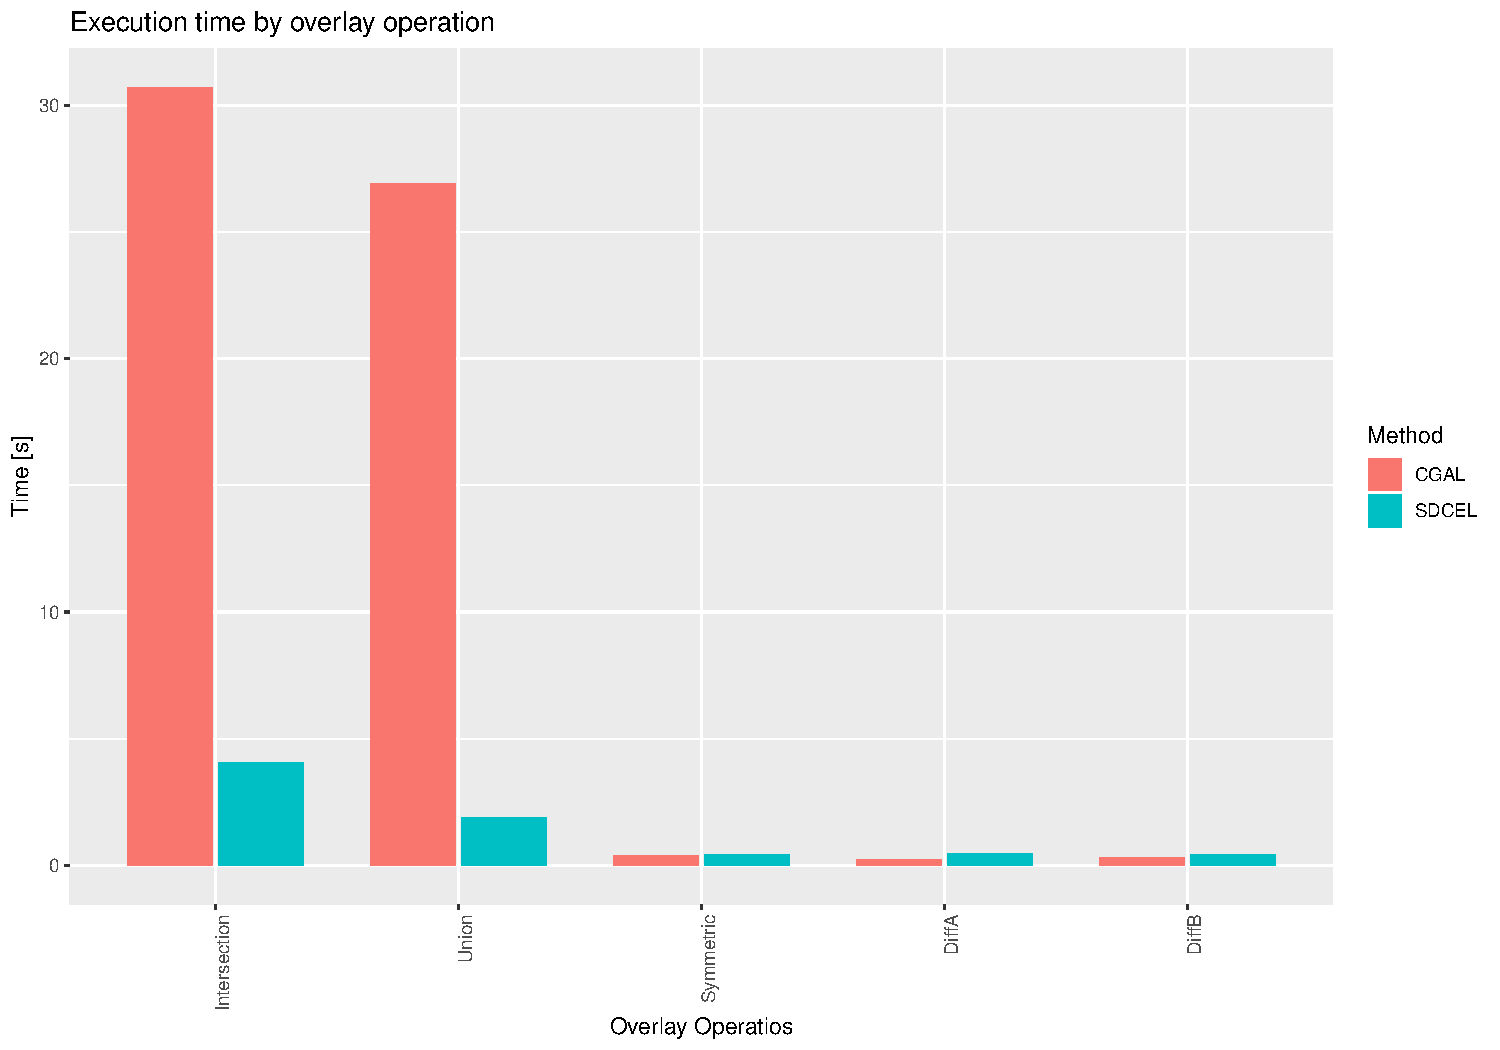
\includegraphics[width=0.8\textwidth]{figures/ByOperators}
\end{frame}

\begin{frame}{Experiment results}
    \centering
    \begin{tabular}{l l l}
        \hline
        Implementation & Operator & Time[s] \\ \hline
        CGAL	& Intersection	& 30.71 \\
        SDCEL	& Intersection	& 4.05 \\
        CGAL	& Union	& 26.92 \\
        SDCEL	& Union	& 1.90 \\
        CGAL	& Symmetric	& 0.38 \\
        SDCEL	& Symmetric	& 0.42 \\
        CGAL	& DiffA	& 0.22 \\
        SDCEL	& DiffA	& 0.45 \\
        CGAL	& DiffB	& 0.30 \\
        SDCEL	& DiffB	& 0.40 \\ \hline
    \end{tabular}
\end{frame}

\begin{frame}{What's next}
    \begin{itemize}
        \item Run additional tests on CA results.
        \item Fix performance issues in SDCEL Symmetric operators.
        \item Still working on load balance in the cluster.
    \end{itemize}
\end{frame}

\end{document}
